\documentclass[final]{acmsiggraph}       % final
%\documentclass[review]{acmsiggraph}      % review
%\documentclass[widereview]{acmsiggraph}  % wide-spaced review
%\documentclass[preprint]{acmsiggraph}    % preprint
%\documentclass[draft]{acmsiggraph}    % preprint

%% Uncomment one of the four lines above depending on where your paper is
%% in the conference process. ``review'' and ``widereview'' are for review
%% submission, ``preprint'' is for pre-publication, and ``final'' is for
%% the version to be printed.

%% The 'helvet' and 'times' packages define the typefaces used for
%% serif and sans serif type in this document. Computer Modern Roman 
%% is used for mathematics typesetting. The scale factor is set to .92
%% to bring the sans-serif type in line with the serif type.

\usepackage{color}
\usepackage{amsmath}
\usepackage{amssymb}
\usepackage{times}
\usepackage{graphicx}
\usepackage{subfigure}
\usepackage{parskip}
\usepackage{fancyvrb}
\usepackage{tabularx}
\usepackage{rotating}
\usepackage{calc}

\newcommand{\IText}[2]{   % #1=Image, #2=Text 2
%  \mbox{#1\hspace{.5\baselineskip}} 
  \begin{turn}{90}
    \parbox{\heightof{#1}}{\centering#2}
  \end{turn}
}

\newcommand{\Rn}[1]{{\mathbb R}^{#1}}
\newcommand{\vect}[1]{\boldsymbol{\mathrm{#1}}}
\newcommand{\mat}[1]{\mathrm{\mathbf{#1}}}
\newcommand{\trans}[1]{#1^{\mathrm{T}}}
\newcommand{\pinv}[1]{#1^\dagger}
\newcommand{\vectt}[1]{\trans{\vect{#1}}}
\newcommand{\trace}[1]{\mathrm{Tr}(#1)}
\newcommand{\ignore}[1]{}
\newcommand{\remark}[1]{\emph{\color{red}#1}}
\newcommand{\x}{\vect{x}}
\newcommand{\y}{\vect{y}}
\renewcommand{\H}{\mat{H}}
\renewcommand{\v}{\vect{\nu}}
\newcommand{\xhat}{\hat{\x}}
\newcommand{\Id}{\mat{I}}
\newcommand{\sigmav}{\sigma_{\v}}
\renewcommand{\t}{\vect{\theta}}
\newcommand{\NN}{\mathrm{NN}}
\def\placeholder#1#2{\fbox{\vbox to #2{\vss\hbox to #1{\hss~}\vss}}}

\onlineid{}

\title{\vspace{-5mm}PaperLess: A Scalable Electronic Receipt Processing System}

\author{Sean M. Arietta and William P. Burns}

\keywords{}

\begin{document}

\maketitle

\remark{Insert abstract here}

%% ACM Computing Review (CR) categories. 
%% See <http://www.acm.org/class/1998/> for details.
%% The ``\CRcat'' command takes four arguments.

%\begin{CRcatlist}
%\end{CRcatlist}

%% The ``\keywordlist'' command prints out the keywords.
% \keywordlist

%\copyrightspace

\section{Introduction}
As the world becomes more environmentally conscious, it becomes
increasingly necessary to revise the financial transaction
infrastructure to accommodate the trend.  Although paper receipts
create very little waste on a per transaction basis, the volume of
receipts being printed daily has a negative effect on the environment.
The Paperless system aims to reduce this wastefullness by providing
customers with the option of receiving a digital receipt in place of
its paper counterpart.  Customers can then access their digital
receipts through the Paperless system via an online web interface,
providing an environmentally friendly alternative to paper receipts
with the added benefeit of a scalable distributed backend capable of
compiling statistical data on customer purchasing activity.

In the initial phase of this project we enumerated a small set of
general goals for the system.  We wanted the system to be invisible to
both the consumer and the seller to minimize both training and
confussion during the transition to the Paperless system.  In
addition, due to the large number of transactions that occur daily, we
knew from the start that the system had to be scalable and would
likely need to be distributed.  Additionally, we imagined that
companies utilizing the system would want to aggregate statistical
data on customer activity.  This would require permanent storage of
the receipts in our digital warehouse.

During the next phase of the project we examined the potential risks
associated with our undertaking and determined what could reasonably
be accomplished in a semester.  Since we did not have direct access to
a functional point of sale (POS) system nor the means to procure one
we decided to focus primarily on the processing and warehousing
aspects of the system. 

In this paper, we discuss the project as it was proposed and the
progress that we have made thus far.  In
Section~\ref{sec:requirements} of the paper we present an overview of
the important requirements for the system and discuss their
significance.  Section~\ref{sec:overview} provides an overview of the
system from a structural perspective.  This section is not intended to
detail the inner-workings of the system but rather the components that
comprise it.  In Section~\ref{sec:implementation}, we discuss our
implementation methodology as it pertains to Software Engineering.
While our goal was to create a functional product, we were primarily
concerned that whatever progress we made over the course of the
semester was accomplished through the use of good Software Engineering
practices. Section~\ref{sec:results} discusses how we tested the
system once it was functional and what we learned from our initial
testing that will be addressed in future
work. Section~\ref{sec:future} addresses our future work on the system
and we conclude the paper in Section~\ref{sec:conclusion} with our
reflections on the overall experience.


\input{overview-fig}

\section{Requirements}

\remark{Define the reqs on the system from a world point of
  view. Discuss the direct printing system and the clearinghouse}


\section{System Overview}
\label{sec:overview}

In this section we present the system-level implementation of our
approach. We describe the various components to our system and
describe the interactions between them. This is not meant to be a
formal specification, but rather a more informal description of our
specific implementation. For a more formal description of our system
please see the supplemental material.

We now describe our system in two parts. The first is the receipt
processing group, which is responsible for receiving, processing, and
saving receipts from customers. The second part of this section
describes the backend data warehousing group. We use this group to
store the receipt data from the processing group for future access and
analysis.

\subsection{Receipt Processing}
\label{sec:overview.processing}

A crucial property of our entire system is that it scale well with
the demands of the customers. As such, our design of the receipt
processing pool reflects this goal. The vision of our system is that
it will able to efficiently and reliably serve many millions of
requests with little or no degradation of service. We set out to
accomplish this by attempting to minimize possible downtime and/or
degradation of service. Our approach is twofold. First, we have
designed our system to be redundant. If any particular subsystem is
faulty for any reason, then our entire system is able to adapt and use
other resources to ``fill in the gaps.'' Unfortunately redundancy is
only half the battle. Even a highly redundant system can fail to
satisfy the needs of a growing number of requests. Therefore, as our
second goal, we wish to create a system that is also highly scalable.

Figure~\ref{fig:overview} is an overview of our system. The entry
point to the entire processing portion is the gateway. All receipt
requests arrive at the gateway. From there, our ProcessDistributor
attempts to schedule the receipt to be processed by a particular
ReceiptProcessingServer. Each receipt is assigned its own thread that
will be responsible for communicating with a particular processing
server. The threads themselves are designed to be lightweight and
completely independent. This allows the gateway to handle a large
number of receipts at once. Although this puts a critical confidence
in the gateway servers, we are able to provide redundancy and
scalability by using a simple scheme that uses DNS to choose an
alternative gateway if one goes down or to simply add a new one to the
pool and add a DNS entry if demand is higher.

One important issue for the gateway is its ability to
load-balance. This is accomplished by keeping a list of recently
scheduled jobs for each server. If a server does not respond to a
request, it is put on a blacklist and another server is used
instead. Periodically the distributor will check its blacklist to see
if any of those servers have come back online. New servers can be
easily added and removed by simply updating these lists allowing us to
easily scale our entire system as needed.

The servers themselves can be run on effectively any hardware with an
Internet connection. The server process simply polls its listening
socket for any connections from the gateway, and upon receiving a
request, processes that request and returns the result. Specifically,
when a processing server receives a request to process a receipt, it
first loads the receipt from a redundant distributed file system,
performs optical character recognition (OCR), parses the result into a
set of lines, and saves the information to our data warehouse.

\subsection{Database Overview}
\label{sec:overview.db}

As previously stated a primary goal of our system is that it is scallable.  To accomodate this requirement on the backend, we elected to run our data warehouse on a MySql Cluster.  The two most appealing aspects of MySql Cluster for our project are that it allows for multiple management nodes and that storage nodes can be added and removed on the fly.  It is essential that in the absence of catastrophic failure our system remains functional.  The system must be able to recover gracefully from errors such as power failures, disk failures, connection failures, etc.  MySql accomodates this necessity by automatically replicating data over storage nodes when a storage node fails to satisfy our desired redundancy.

In accordance with our requirement that there be no single point of failure in our system we decided that a distributed architecture was essential.  We have designed the system such that the data warehouse consists of multiple geographically separated locations which together represent the entire database.

Another crucial aspect of the MySql cluster is that it load balances automatically.  This was a major benefeit for our project because while we wanted to develop a system that was customized to our needs, we didn't want to re-invent the wheel.  We believe that any issues regarding load-balancing in MySql Cluster are low-risk.  If load balancing becomes an issue, it can be resolved easily by adding more management and storage nodes.  It may not be an elegant solution, but commodity hardware is cheap and the benefeit of developing a custom load balancer to suit our needs does not outway the effort and time required to do so.


\section{Implementation}
\label{sec:implementation}

In the spirit of good software engineering practices we made every
effort to abide by a rigorous approach during development. The outcome
of our efforts was a similar, but slightly tailored version, of the
agile method. We dub our method rapid collaborative refinement. In
essence, due to our small development team (2), close proximity, and
unqiue abilities we were able to very quickly refine a particular
piece of code or refine our approach by alternating between personal
interaction and separated investigation. The lifecycle for a
particular system-level decision was therefore reduced to a small
overhead leaving us more time to focus on developing useful software
and well-constructed software. This approach is depicted graphically
in Figure~\ref{fig:RCR}. Notice that we are able to more tightly close
the loop on developing a particular aspect of the system due to our
methodology.

Our development environment consisted of several testing machines
running Linux and Mac OS X, the Eclipse IDE, git source code
management through github.com, mySQL Cluster Server, and MyEclipse for
making logical diagrams. All code was written in JAVA so that we
would have more flexibility in deplyoment options.

We know describe in detail the actual software behind our system. In
Section~\ref{sec:overview} we discussed the high-level overview of our
system. Now we will explain exactly what we did, and what we didn't
do. We will start by describing our implementation of the processing
group and then move on to the data warehousing group.

\subsection{Processing Group}
\label{implementation.processing}

From a high-level perspective, the processing group is responsible for
processing a set of receipts in an efficient and scalable manner. For
this reason we chose to separate the role of process assignment and
process fulfillment. Our ProcessDistributor acts as the assigner. It
polls its listening socket and waits for a request to process a
receipt. When it receives a request, it simply puts the request into a
FIFO queue. A separate thread continuously checks the queue for
elements and upon finding one creates a new handling thread that will
process the item.

Each handling thread executes a remote procedure call (RPC) to a
ReceiptProcessingServer. The particular server chosen is determined by
the ProcessDistributor and is currently just a round-robin
selection. The RPC itself was written from scratch so that we would
have the flexibility to create a lightweight object tailored to our
very simple needs. RPC's are implemented as serializable objects that
can be transferred via a socket to a ReceiptProcessingServer. Upon
receiving the RPC, the processing server extracts the necessary
information from the parameter field, saves the relevant data to the
mySQL backend (see Section~\ref{sec:implementation.db}), and then
returns a response.

As discussed in Section~\ref{sec:overview.processing} our goal was to
be able to process imags of receipts. These images would be stored on
a distributed file system and the RPC parameters would just consist of
a file handle to the particular receipt image to be processed. Due to
complications, we were unable to accurately perform OCR on
images. Section~\ref{sec:results} describese in more detail exactly
what these complications were. Nevertheless, we still wanted to
implement a working system if not complete. In our current
implementation, the parameter to the RPC is a string representation of
a receipt. Our system then parses the string representation (just as
it would parse the output of OCR) for the item name, price, quantity,
seller, user information, etc. This information is saved to our mySQL
cluster database through the JAVA mySQL connector.

If at any time there is an error on the processing server, a message
is sent bck to the distributor notifying it of the error. The
distributor is then able, depending on the error, to re-queue the
receipt for processing again. Some situations where this would be
appropriate would be if the processing server happens to lose
connectivity with the mySQL database.

The beauty of the system is that independent functional parts are
separated by logical and information boundaries. The distributor knows
only a list of possible processing servers. It holds the queue and
iteratively attempts to empty the queue by sending RPC's through its
handling threads to a processing server. The processing servers, in
turn, know nothing about the distributor. They simply listen for data
on their sockets, process requests that come to them, and return the
results. Similarly the database has no knowledge of the specifics of
neither the processing servers nor the distributor. This setup allows
us to very easily scale the entire operation as needed. We need only
notify the distributor that another potential processing server is
available. All other parts are completely agnostic to its pressence or
lack thereof.

\subsection{Data Warehousing Group}
\label{sec:implementation.db}

\remark{Fill in details about the actual implementation of the database group. Include specifics about libraries, schema, etc. DO NOT include information regarding any results. We have a separate section for that :)}

\section{Results}
\label{sec:results}

Our goal was to create a system that could process receipts in a
scalable and reliable way. We have defined scalability as the ability
to quickly and seemlessly add or remove processing
entities. Reliability refers to the persistance of data after it has
been received by our system. We have described our system and its
specific implementation to date in Section~\ref{sec:overview} and
Section~\ref{sec:implementation}. Now we set out to evaluate our work.

First we will consider scalability. In order to test the scalability
of our system we required a large test set. As mentioned in
Section~\ref{sec:implementation.processing}, we were unable to get
adequate results from an optical character recognition package we
tried. We tried Tesseract and SimpleOCR on a small set of test
receipts. Although according to 1995 UNLV Accuracy Test, Tesseract is
one of the best OCR packages available. However, our initial tests
deemed it unable to extract text correctly from receipts most likely
due to the poor resolution available and the non-standard layouts
present in receipts from many different companies. Therefore, we chose to consider receipts as strings with fields corresponding to what would have been extracted from an OCR package. A typical receipt line then takes the form:

\begin{centering}
\{receipt:RECEIPT ID\} \{item: ITEM NAME\} \{price: ITEM PRICE\} \{quantity: QUANTITY\} \{store: STORE ID\} \{date: PURCHASE DATE\}
\end{centering}

For our tests, we generated 30,000 lines of this format. We then
wrote a simple test harness that looped over the list and sent each
line to the process distributor gateway. We ran this test with three
processing servers available. The bottleneck in the system is the
distributor. It receives all of the requests nearly simultaneously and
must federate them off to individual threads while maintaining a queue
of the non-processed receipts. In a setting where there are hundreds
of thousands of receipts coming in at once, this can become a
burden. However, even with a modest hardware configuration consisting
of a MacBook Pro with 2GB of RAM and a 2.16GHz Core2 Duo we were able
to handle 30,000 requests arriving nearly simultaneously. 

We also ran tests to assess the ability for our system to adapt to new
or failed servers. We began by running the same test as before but in
the middle of the test we killed off a node. The distributor was able
to distribute the receipts effectively across the remaining servers in
the pool. Likewise, if we added a new server, the disitrbutor was able
to adapt and send receipts to the newly added one too. Our tests show
that we have indeed created an effective receipt processing system
that can be scaled to meet demand.

Since one of our goals was to develop our system in line with standard
Software Engineering practice we also provide results for our logical,
infrastructure, and use case diagrams. These are included in Appendix
A.


\section{Future Work}

\remark{How we envision the system behaving in the future. Mention the
  possibility of interfacing with the POS system directly OR (and I
  think this is important), how we might improve the OCR package
  ourselves. In a sense we kind of know what we're looking for when we
  OCR a receipt.}


\section{Conclusions}

\remark{Conclusion}

\bibliographystyle{acmsiggraph}
\bibliography{paper}

\begin{figure*}[t]
\centering
\def\imw{1.0\textwidth}
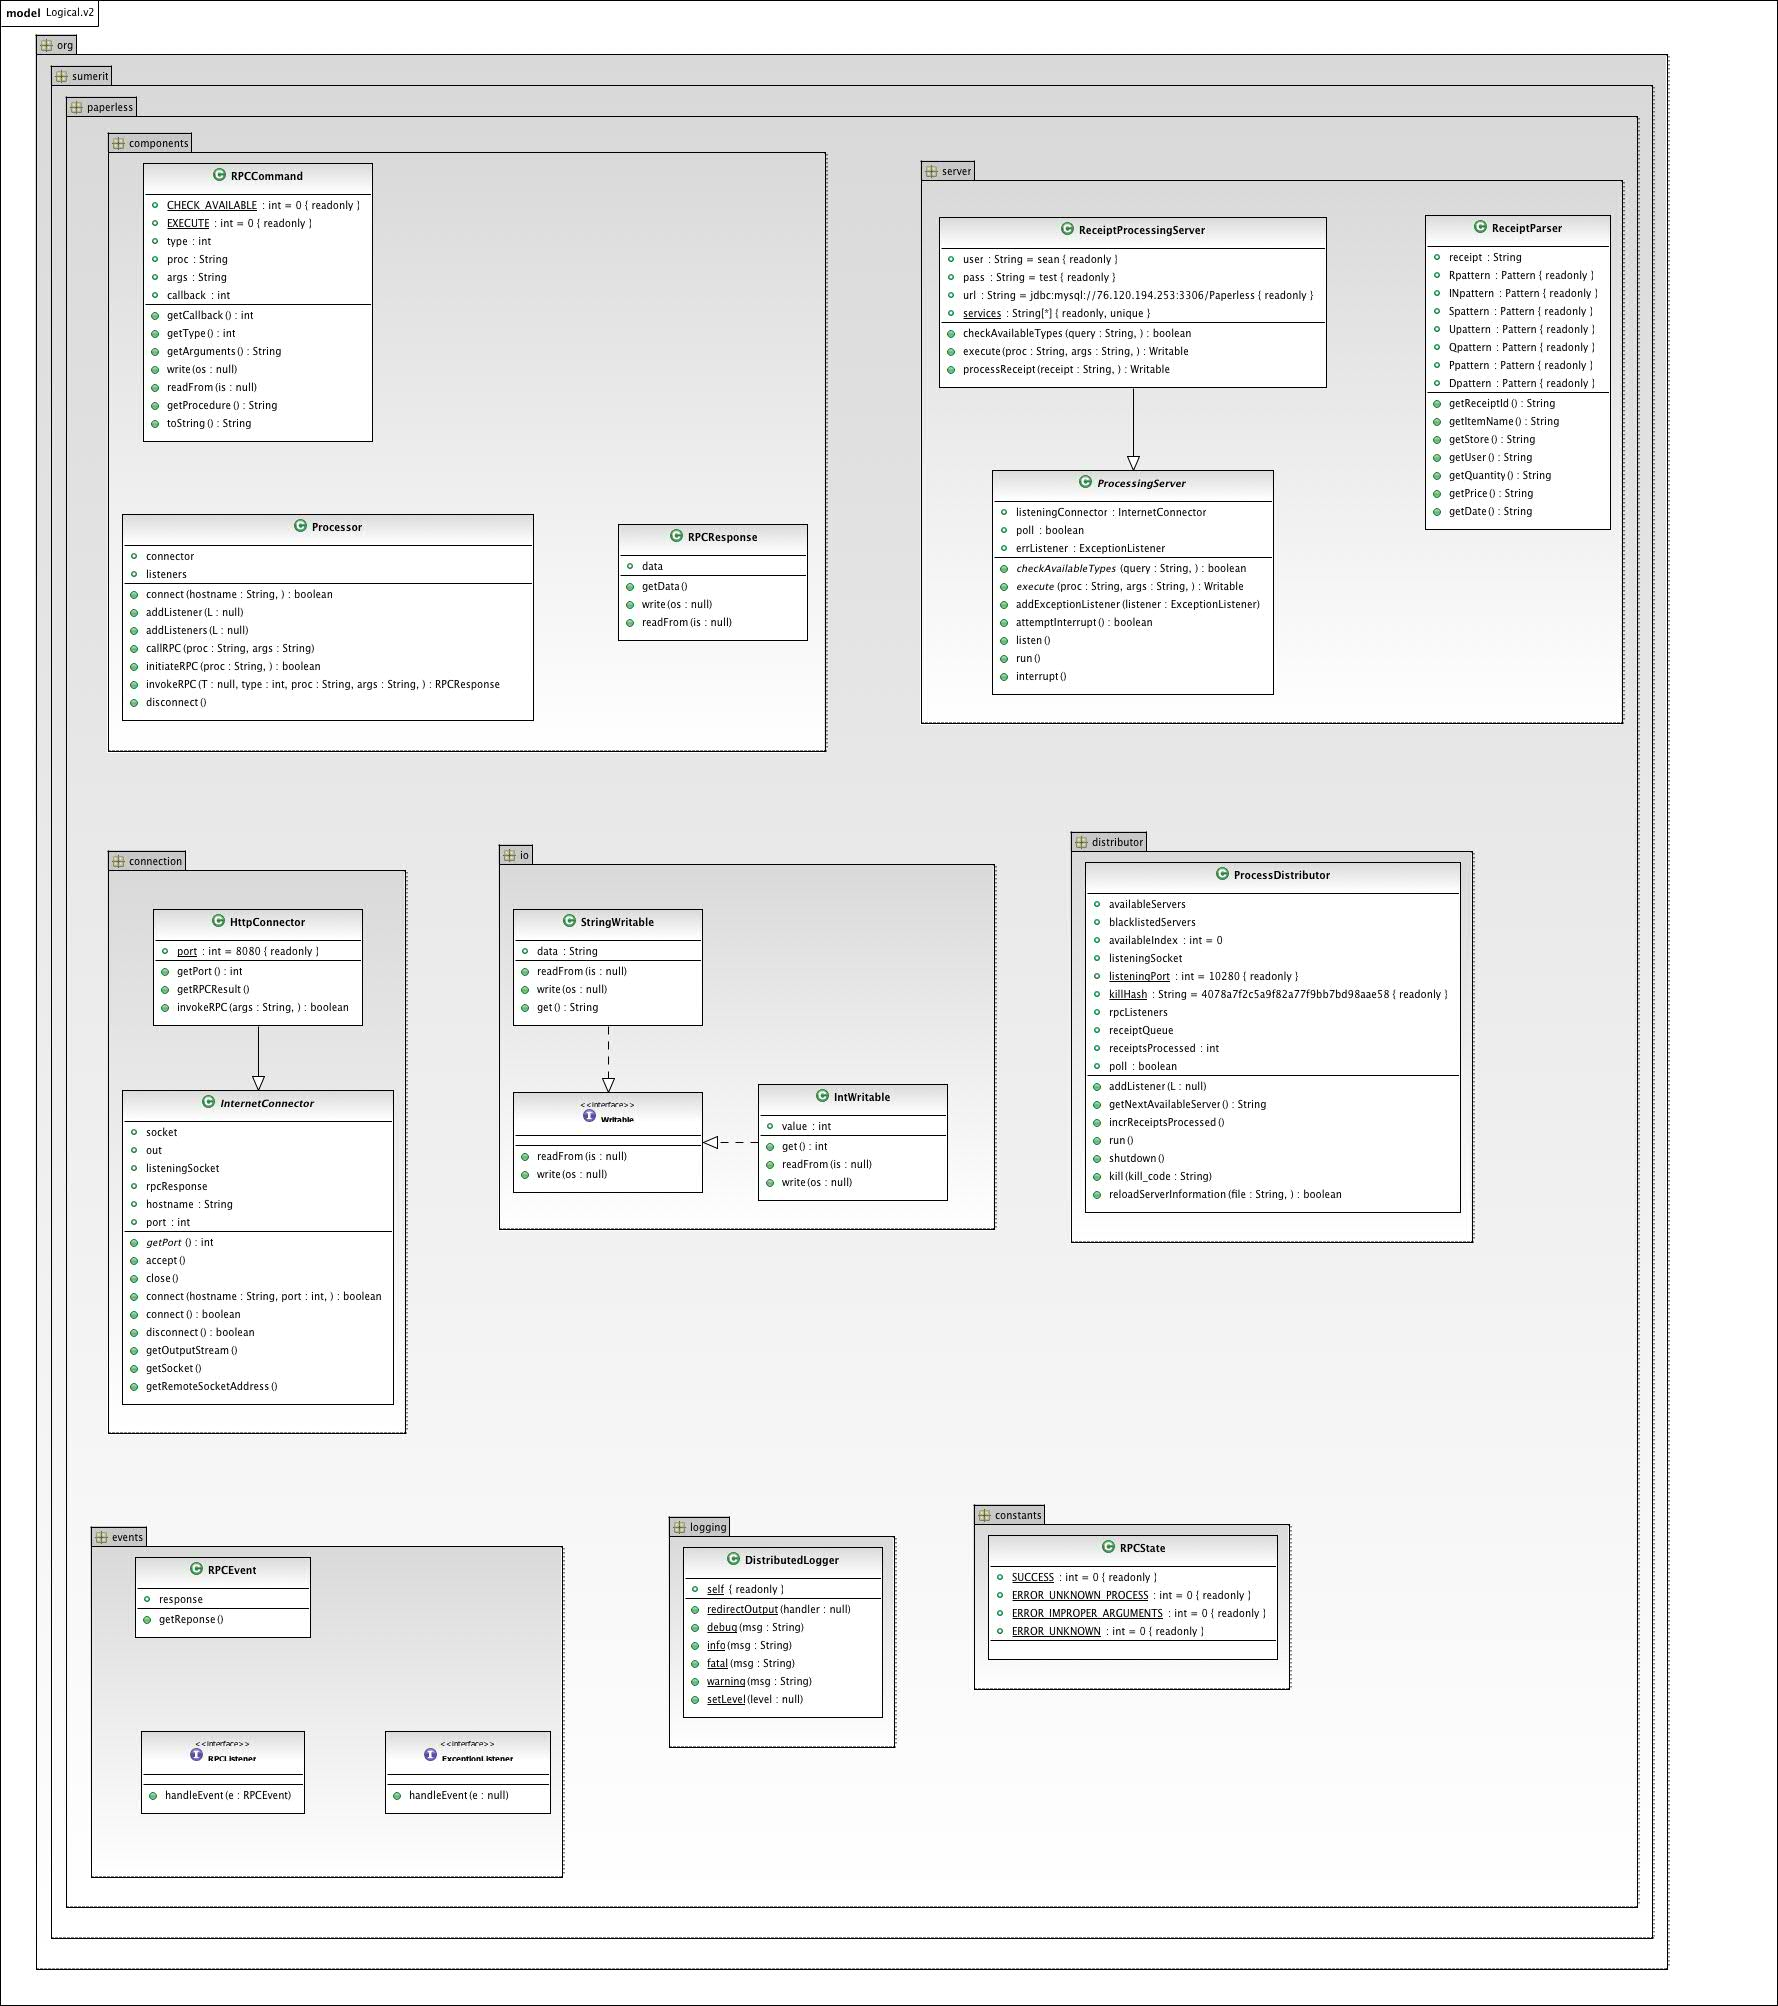
\includegraphics[width=\imw]{figs/logical.png}\vspace{-3mm}
\caption[]{\textbf{Logical View} Shows the UML diagram of our processing software package.}
\end{figure*}

\begin{figure*}[t]
\centering
\def\imw{1.0\textwidth}
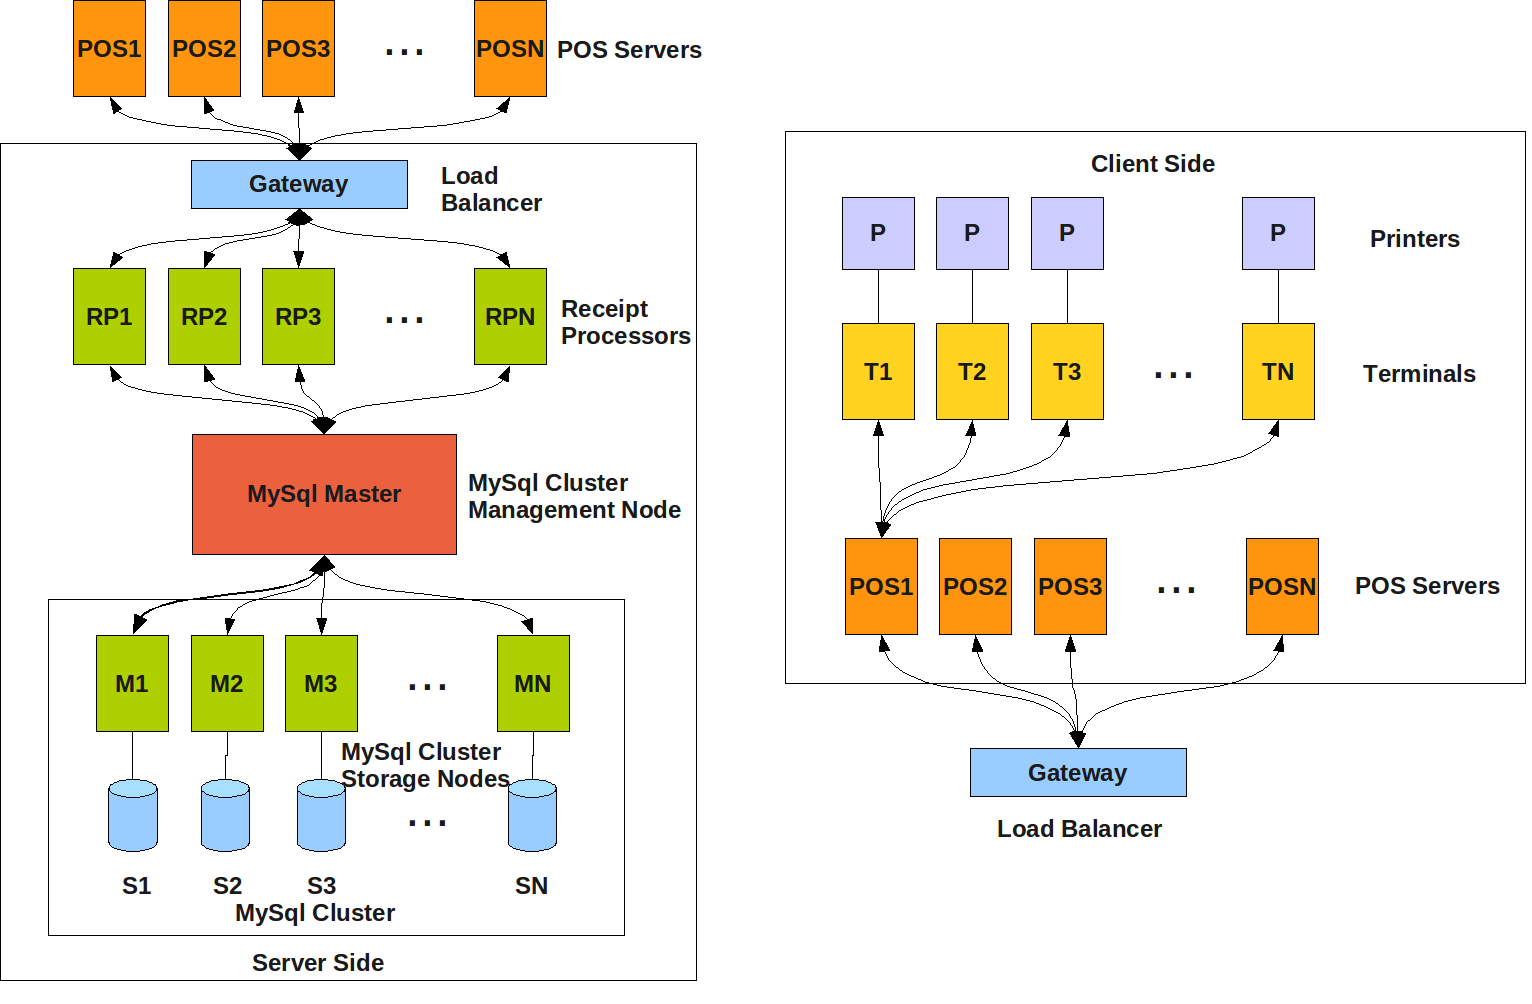
\includegraphics[width=\imw]{figs/infrastructure.png}\vspace{-3mm}
\caption[]{\textbf{Infrastructure View} Shows the components and the connections between components of our system}
\end{figure*}

\begin{figure*}[t]
\centering
\def\imw{1.0\textwidth}
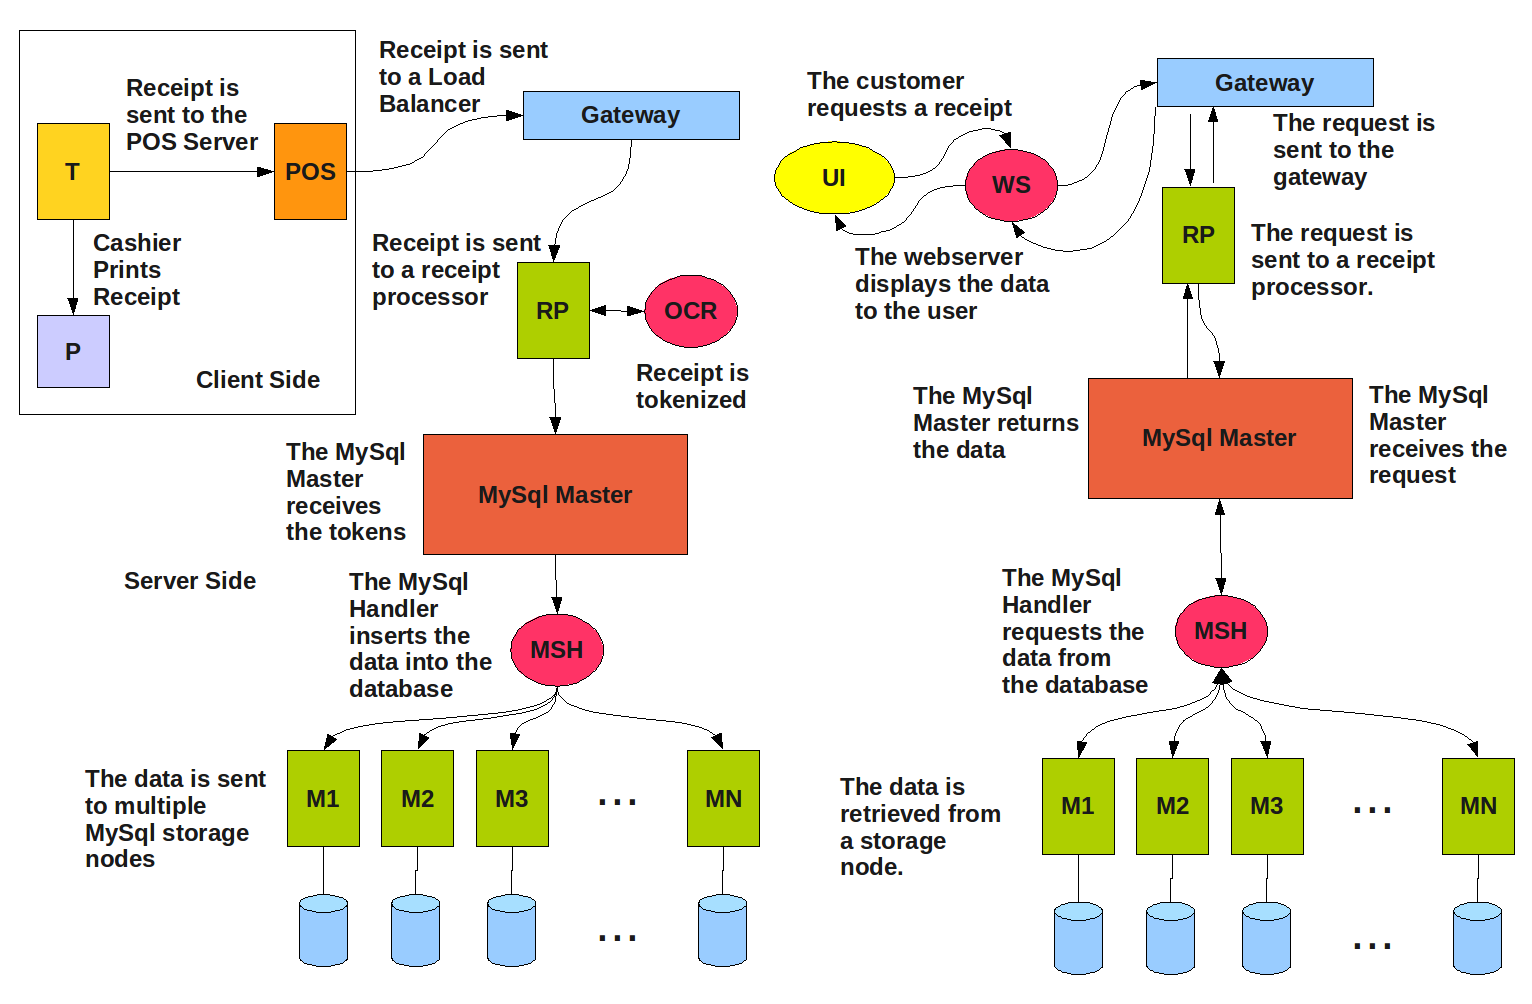
\includegraphics[width=\imw]{figs/usecases.png}\vspace{-3mm}
\caption[]{\textbf{Use Cases} Some typical use cases from both the seller and consumer points of view}
\end{figure*}

\end{document}
\package{}
